\documentclass[a4paper, 12pt]{article}
\usepackage[slovene]{babel}
\usepackage[utf8]{inputenc}
\usepackage[T1]{fontenc}
\usepackage{lmodern}
\usepackage{graphicx}
\usepackage{amssymb}
\usepackage{amsmath}
\usepackage{mathtools}
\setlength{\parindent}{0px}
\setlength{\parskip}{10px}
\usepackage{enumitem}
%\usepackage{blindtext}
\usepackage{lipsum}
\usepackage{scrextend}
\usepackage{array}
\usepackage{tikz}
\usepackage{pgfplots}
\usetikzlibrary{patterns}
\pgfplotsset{width=7cm, compat=1.10}
\usepgfplotslibrary{fillbetween}
\usepackage[margin=1in]{geometry}
\usetikzlibrary{shapes,arrows}
\usepackage{listings}
\usepackage{color}
\usepackage{multirow}
\usepackage{caption}
\usepackage[
colorlinks=true,
linkcolor=black,
anchorcolor=black,
citecolor=black,
filecolor=black,
menucolor=black,
runcolor=black,
urlcolor=black
]{hyperref}

\title{Zapiski iz pouka Osnove programiranja II Programiranje Mikrokontrolerjev}
\author{Matej Blagšič}

\begin{document}

%---------------------------------------------------za diagrame
\tikzstyle{decision} = [diamond, draw, fill=blue!20, 
text width=4.5em, text badly centered, node distance=3cm, inner sep=0pt]
\tikzstyle{block} = [rectangle, draw, fill=blue!20, 
text width=5em, text centered, rounded corners, minimum height=4em]
\tikzstyle{line} = [draw, -latex']
\tikzstyle{cloud} = [draw, ellipse,fill=red!20, node distance=3cm,
minimum height=2em]
\tikzstyle{nothing} = [draw, node distance =3cm]

%-------------------------------------za programiranje text barvanje
\definecolor{dkgreen}{rgb}{0,0.6,0}
\definecolor{gray}{rgb}{0.5,0.5,0.5}
\definecolor{mauve}{rgb}{0.58,0,0.82}
\definecolor{lgray}{RGB}{250,250,250}

\renewcommand\lstlistingname{Program}
\renewcommand\lstlistlistingname{Program}
\def\lstlistingautorefname{Alg.}

\lstset{
	frame=l,%single
	language=[ANSI]C,
	aboveskip=3mm,
	belowskip=3mm,
	showstringspaces=false,
	columns=flexible,
	basicstyle={\small\ttfamily},
	numbers=none,
	numberstyle=\tiny\color{red},
	keywordstyle=\color{blue},
	commentstyle=\color{dkgreen},
	stringstyle=\color{mauve},
	breaklines=true,
	breakatwhitespace=true,
	tabsize=4,
	backgroundcolor=\color{lgray},
	moredelim=**[is][\color{dkgreen}]{@}{@},
}

\lstdefinestyle{customc}{
	belowcaptionskip=0.5\baselineskip,
	breaklines=true,
	xleftmargin=\parindent,
	language=C,
	showstringspaces=false,
	basicstyle=\footnotesize\ttfamily,
	keywordstyle=\bfseries\color{green!40!black},
	commentstyle=\itshape\color{purple!40!black},
	identifierstyle=\color{blue},
	stringstyle=\color{orange},
}

\lstdefinestyle{customasm}{
	belowcaptionskip=0.5\baselineskip,
	xleftmargin=\parindent,
	language=C,
	basicstyle=\footnotesize\ttfamily,
	commentstyle=\itshape\color{purple!40!black},
}

\lstset{escapechar=@,style=customc}

%---------------------------------------//

\newcommand{\harpoon}{\overset{\rightharpoonup}}


\maketitle
\thispagestyle{empty}
\pagebreak
\setcounter{page}{1}

\tableofcontents
\pagebreak

\section{Programiranje v C}

\subsection{Osnovno}

Pri temu predmetu bomo obravnavali jezik C. Za uporabo lahko preneseš okolje Codeblocks z MinGW inštalacijo ali posebej MinGW compiler in poljubno okolje(Jetbrains).\

Pomembno je, da imaš predznanje iz prejšnjega polletja pri Javascriptu, saj so tipi spremenljivk, sintaksa in drugo zelo podobno, tako da v detajle o stvarih, ki so enake ne bom šel.

Vsak dokument začnemo z \framebox{\lstinline|@#include <stdio.h>@|\par} za standardne vhodne in izhodne ukaze.

Vsa koda se izvaja znotraj main funkcije:

\begin{lstlisting}
int main(){
    printf("Hello!\n");
    return 0;
}
\end{lstlisting}

\textbf{Prav tako je pomembno uporabiti PODPIČJE za vsakim ukazom/vrstico!!!}

Če začnemo na začetku, opazimo \texttt{\#include} ukaz. Ta se izvrši, preden se karkoli drugega. V temu primeru lahko vnesemo knjižnice. Te nam olajšajo programiranje s tem, da nam en ukaz izvede več ukazov, ki bi jih morali tipkati na roke. To datoteko/knjižnico navedemo lahko z "datoteka" navednicam. Če pa damo v <datoteka>, potem pa išče datoteke v sistemskih mapah okolja. Te datoteke so vrste \textbf{header} s končnico \textbf{.h}. V našem primeru je knjižnica za pisat in brat podatke - vhodne in izhodne podatke.\\
To je podobno kot v javascriptu:  \lstinline|<script src="datoteka">|\ 
\subsection{Podatki}
Poglejmo si zgled:
\begin{lstlisting}[caption = Branje in pisanje podatkov]
int main(){
	int a;
	float b; //spremenljivka

	printf("Vprisi prvo vrednost");
	scanf("%d", &a);
	printf("Vpisi drugo vrednos");
	scanf("%f", &b);
	printf("%d + %f = %f\n", a, b, a+b);
	return 0;
}
\end{lstlisting}

C je občutljiv na tip podatkov. Pravimo tudi, da je C statično tipiziran jezik. To pomeni, da moramo vrsto podatka navesti. 
To pomeni, da se moramo sami odločiti, kakšen tip podatka bo nosila spremenljivka.

Vemo, da v Javascriptu nismo rabili napisati tipa spremenljivke, le \texttt{var}, torej je Javascript dinamično tipiziran jezik.

\subsubsection{Branje podatkov}
Da nam program prebere podatek, uporabimo funkcijo:

\begin{center}
	\framebox{\lstinline|scanf("formatno\_dolocilo", \&spremenljivka);|}
\end{center}

Vidimo, da moramo najprej deklarirati tip podatka, ki ga pričakuje operator Scanf. Potem pa določimo naslovni operator \& in nato za njim spremenljivko, ki naj sprejme podatek.

Še eno " pravilo scanf funkcije. Funkcija dejansko vrne število. To kar vrne je odvisno od "uspeška" funkcije. Vrne lahko 2, če so bili vhodni podatki pravi. Vrne 1, če je bil en podatek mal napačen. Vrne 0, če je bil en podatek čisto napačen.

\subsubsection{Pisanje podatkov}
Za pisanje podatkov uporabimo funkcijo:
\begin{center}
	\framebox{\lstinline|printf("formatni\_niz", izrazi)|}
\end{center}
Pomembne so tudi ubežne sekvence. To so \verb|\r \n \t|, ki povejo, kaj se zgodi, ko se text izpiše. \verb|\n| naredi novo vrstico(new line) po besedilu, \verb|\t| je tabulator...

Tako v našem primeru, se a izpiše tam, kjer je njegov \verb|%d| in b, kjer je \verb|%f| ter vsota $a + b$ tam, kjer je \verb|%f| (glej izsek programske kode).

\subsubsection{Spremenljivke:}
\begin{table}[!htbp]
	\centering
	\begin{tabular}[b]{|p{3cm}|p{3cm}|p{3cm}|p{4.5cm}|}
		\hline \textcolor{blue}{TIP} & \textcolor{blue}{DOLŽINA(bitov)} & \textcolor{blue}{FORMATNO DOLOČILO} & \textcolor{blue}{OBMOČJE} \\ \hline\hline
		\textcolor{violet}{char} & 8 & \verb|%d %c| & $-128$ do $127$ \\
		\multirow{2}{*}{\textcolor{violet}{short, int}} & 16 & \multirow{2}{*}{\texttt{\%d}} & $-65536$ do $+65535$ \\
		& 32 && $-32768$ do $+23767$ \\
%		32  & \%d &$-65536$ do $+65535$ \ $-32768$ do $+23767$\\
		\textcolor{violet}{long} & vsaj 32 & \verb|%ld| & $-2.1\times10^9$ do $+2.1\times10^9$\\
		\textcolor{violet}{float} & običajno 32 & \verb|%f| & $-2.1\times10^9$ do $+2.1\times10^9$\\
		\textcolor{violet}{double} & običajno 64 & \verb|%lf| & $-9.2\times10^{18}$ do $+9.2\times10^{18}$ \\
		\textcolor{violet}{void} & 0 & & \\ \hline
	\end{tabular}
	\caption{Tipi spremenljivk v c-ju}
\end{table}
%
V C-ju Boolov tip ne obstaja, tako da primerjalni operatorji delujejo enako, le da vračajo 0 za false in 1 za vse, kar je različno od nič. \textbf{Ne obstaja TRUE ali FALSE}.\

Spoznali bomo tudi, da je pri celoštevilskem tipu pomembna omejitev območja, pri realnem tipu pa natačnost!

Velikokrat bomo srečali izraz \lstinline|unsigned|. ta nam območje podatkovnega tipa prestavi od 0 do $2\times$ maksimum. Če je char od -128 dp 127, potem je unsigned char od 0 do 255;

\subsubsection{Celoštevilski tip (n bitov)}
Obstaja nepredznačen, ki je od 0 do $2^{32}$

\subsubsection{Realni tip (IEEE floating point)}
\begin{table}[!htbp]
	\centering
	\begin{tabular}{|l|l|l|}
		\hline \textcolor{blue}{p} & \textcolor{blue}{eksp. (e)} & \textcolor{blue}{mantisa (m)} \\ \hline
		1 bit & 8 bitov & 23 bitov \\ \hline
	\end{tabular}
\end{table}

Ta ima enojno natančnost (single precision) ali \emph{\texttt{float}} in so števila zapisana z 32 bitno velikostjo. Tako so v desetiškem sistemu števila natančna do 7,22 signifikantnih mest, sepravi 7 mest je natančnih, od 8. števila naprej pa je že vprašljivo. Torej, signifikantno pomeni pomembno, tisto, kar je natančno.\

Če hočemo večjo natančnost, uporabimo \emph{\texttt{double}} oz. dvojna natačnost (double precision). Ima kapaciteto 64 bitov, torej v desetiškem do 15,95 mest natančno. Po 15. mestu je že vprašljivo natančno.


\subsubsection{Modifikatorji formatna določila}
\verb|%d| vemo, da stoji za cela števila. Če vrinemo neko število ``N'' $\to$ \texttt{"\%Nd"}, potem povemo, na koliko mest se izpiše število, deluje na desno poravnavo.\\
Če vrinemo ničlo $\to$ \texttt{"\%0Nd"}, potem zapolne prazna mesta z ničlam.\\
Če vrinemo "N.Mf" $\to$ \texttt{"\%N.Mf"}, potem izpiše $N$ mest število z $M$ mesti za decimalno piko.

\begin{lstlisting}
int x = 15;
float y = 3.141592;

printf("%5d",x); --> Izpise _ _ _1 5
printf("%.2f",y); --> Izpise 3.14
printf("%05d",x); --> Izpise 00015
\end{lstlisting} 

\subsubsection{Znaki}
Imamo več standardov znakov. Najbolj osnoven in razširjen je \texttt{ASCII} (American standard code for information Interchange). Ta zapis je 8-biten. Lahko najdemo tabelco, ki nam pokaže kodo za vsak znak.

\begin{figure}[h!]
	\centering
	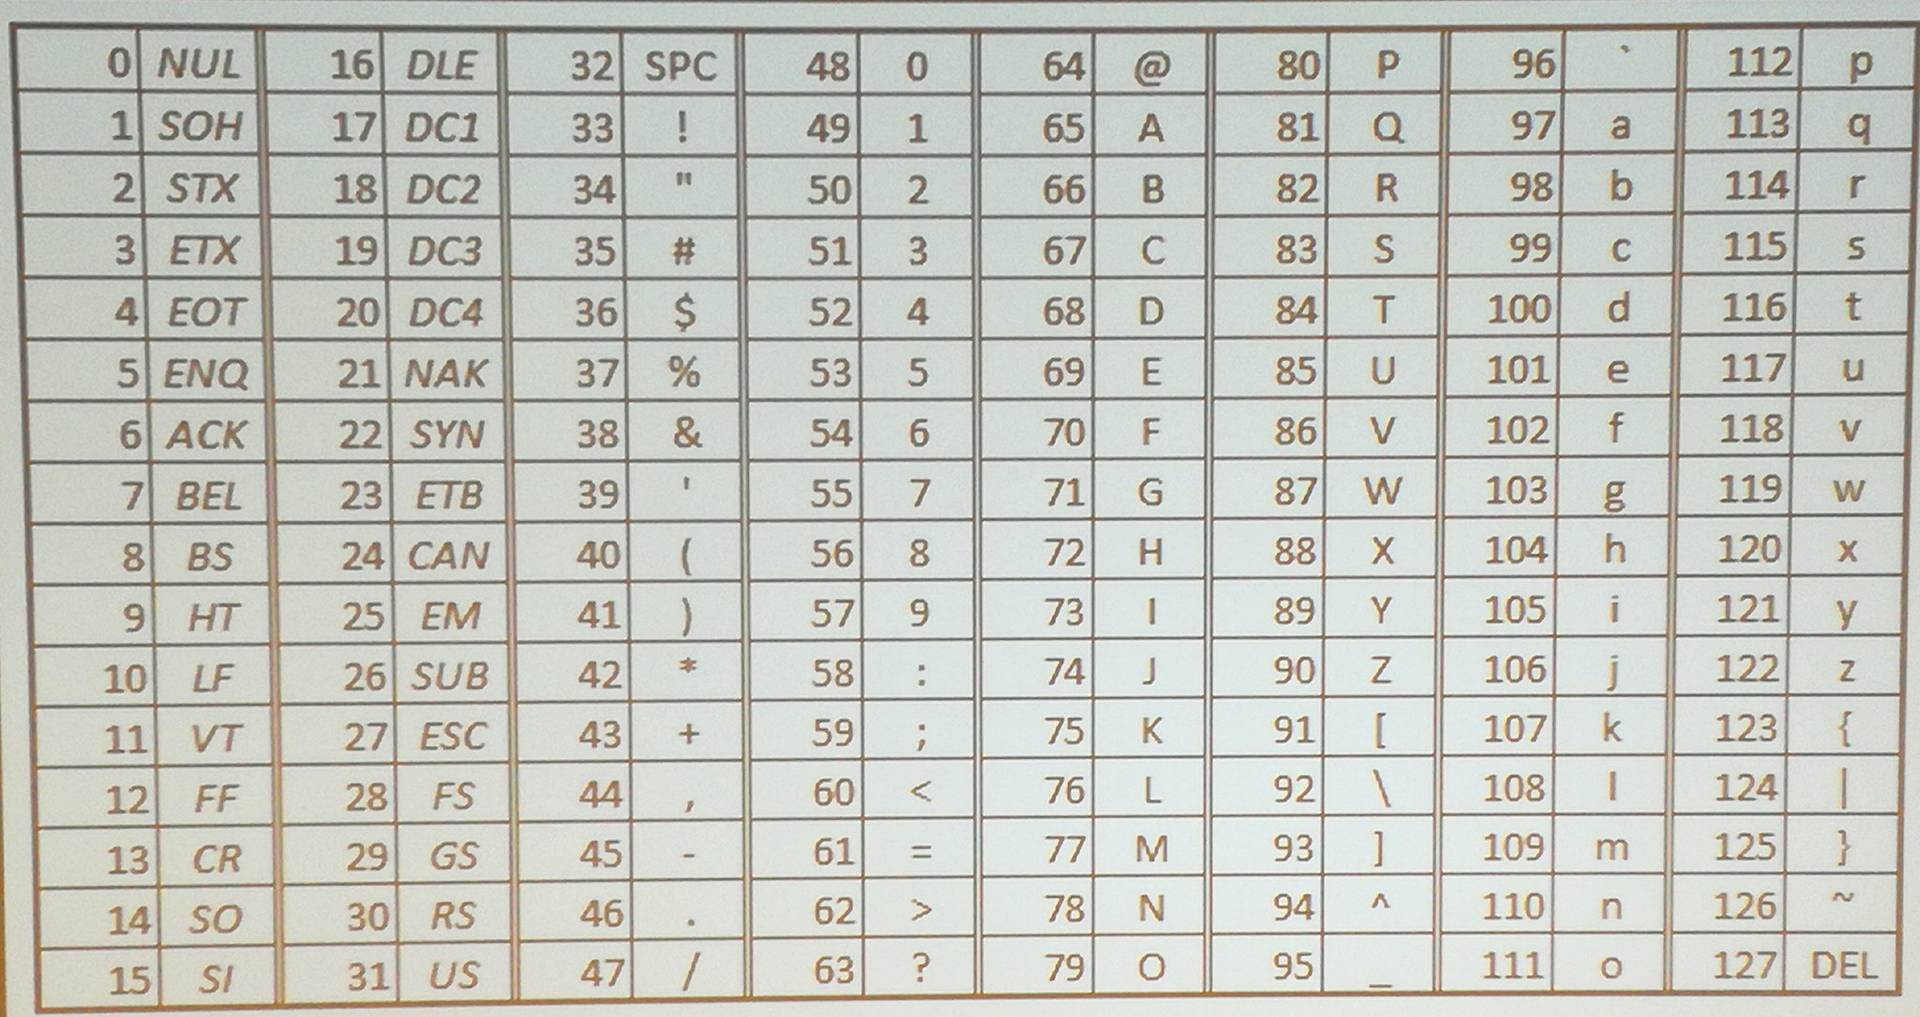
\includegraphics[width=0.7\linewidth]{images/ascii.jpg}
	\caption{ASCII tabela}
	\label{fig:ascii-tabela }
\end{figure}

V C-ju je pomembno, da damo en znak v enojne navednice. S tem pomeni, da program zaznava ASCII kodo. Torej, če izpišemo \lstinline|printf("%d", '0');|, nam program izpiše 48. Pri znakih uporabimo torej spremenljivko \lstinline|char|.

\begin{lstlisting}
int main(){
char x = 130;
char y = -126;
if(x==y) printf("%s", "enako");
return 0;
}
\end{lstlisting}
Koda nam izpiše da je enkao, ampak te dve števili nista enaki. Zakaj potem program reče, da je enako. *ljudje ki so se ukvarjali z neksončnostjo so pristali v inštitucijah*\\
To prihaja zaradi prevelikih števil oz. overflow. Char je 8-bitna spremenljivka, torej vrednosti od -127 do 127 ali 0 - 255. Če zahtevamo število unsigned char recimo 260, to število znotraj char ne obstaja. Zato števec se obrne in gre nazaj na 4.\

Če želimo v c napisati število v 16-iškem(HEX) sistemu, se orientiramo po tabelci iz binarnega v 16-iški sistem:

\begin{table}[!h]
	\centering
	\begin{tabular}{|l|l|l|l|l|l|}
		\hline BINARNO &DECIMALNO &HEX & BINARNO &DECIMALNO &HEX\\
		\hline 0001 & 1&0x1& 1010 & 10&0xa\\
		\hline 0010 & 2&0x2& 1011 & 11&0xb\\
		\hline 0011 & 3&0x3& 1100 & 12&0xc\\
		\hline 0100 & 4&0x4& 1101 & 13&0xd\\
		\hline 0101 & 5&0x5& 1110 & 14&0xe\\
		\hline 0110 & 6&0x6& 1111 & 15&0xf\\
		\hline 0111 & 7&0x7&&&\\
		\hline 1000 & 8&0x8&&&\\
		\hline 1001 & 9&0x9&&&\\  \hline
	\end{tabular}
\end{table}



\subsubsection{Psevdonaključna števila}
Ena metoda za pridobivanje naključnih števil je metoda srednjih kvadratov.
Pri tem kvadriramo dvomestna števila. Pri tem je statistično gledano naključnost zelo podobna realni naključnosti, kot da bi metali kocke.

\subsubsection{Statične in dinamične spremenljivke}
\textbf{Glej priloženo kodo spodaj!}

V temu programu imamo funkcijo tipa void, ki kot vemo ne vrne nič, pred funkcijo main. prav tako imamo definirano spremenljivko ga, ki je zunaj kode. Ta je zato globalna in je uporabna v vseh funkcijah. Te globalne spremenljivke so \textbf{STATIČNE}. To pomeni da so te spremenljivke vedno na voljo in hranijo vrednost ves čas, kajti prostor za njih je že rezerviran v začetku.

Za kontrast, vse lokalne spremenljivke so \textbf{DINAMIČNE}, razen če so definirane kot statične z ukazom \lstinline|static| pred definicijo spremenljivke(glej kodo, vrstica 6). Če poženemo kodo vidimo, kako deluje ukaz static. Ker smo spremenljivko \textcolor{purple}{sa} definirali le enkrat in ji dodali vrednost 12, potem se ne definira ponovno vsakič, ko pridemo v to funkcijo \textcolor{green}{foo()} še enkrat. Zato se vrednost te spremenljivke povečuje. Za kontrast, spremenljivka \textcolor{purple}{a} se ne povečuje, saj se vsakič, ko pridemo v funkcijo \textcolor{green}{foo()} ponovno definira.

Prav tako velja, da statične neinicializirane spremenljivke dobijo vrednost 0. To ne velja za dinamične, tako da če ne zapišemo začetne vrednosti spremenljivke \textcolor{purple}{a}, potem vidimo, da program meče za vrednosti \textcolor{purple}{a} kar nekaj.

\pagebreak

\begin{lstlisting}[caption = Statične in dinamične spremenljivke]
#include <stdio.h>
int ga; //globalna spremenljivka

void foo(){
	int a = 12;	//lokalni spremenljivki
	static int sa = 12; //spremenljivka je staticna
	a++;
	sa++;
	ga++;
	printf("%d, %d, %d\n", ga, a, sa);
}
int main(){
	for(int i=0; i < 5; i++){
		foo();
	}
	return 0;
}	
\end{lstlisting}
\subsubsection{Zbirka(array)}
Pomnilnik je razdeljen na pomnilniške celice v velikosti 8 bitov na celico. Ko naslavljamo celico, je vedno naslednja celica za 1 večja od prejšne po vrstni številki. \

\begin{center}
	\framebox{\lstinline|tipElementa imeZbirke[dim] = \{element1, element2, element3, ...\}|}
\end{center}

V temu primeru, je ,,dim'' dimenzija zbirke. Naslavljamo jih lahko enako, kot v javascriptu, to je, da napišemo ime zbirke in "stevilo, ki predstavlja mesto želenega elementa. Ne moremo izpisati celotne zbirke naenkrat, temveč le po en element naenkrat. Pomembno je tudi, da ena zbirka določenega tipa lahko vsebuje elemente le tega tipa, torej vsi enaki. Ne moremo mešati različnih tipov, kot v javascriptu.

Poglejmo si zanimiv primer:

\begin{lstlisting}
#include <stdio.h>

int a[] = {2, 4};
int b[] = {1, 3};

int main(){

	a[2] = 42;
	b[-1] = 42;

	printf("%d, %d", a[1], b[0]);

	return 0;
}
\end{lstlisting}

V tem primeru, imamo globalna arraya $a$ in $b$. Imata dva elementa, torej je njuna velikost 2. Nato pa v main funkciji elementu 2 v arrayu $a$ in elementu -1 v arrayu $b$ priredimo vrednost 42. In potem, ko izpišemo drugi člen arraya $a$ in prvi člen arraya $b$, se nam izpišeta točno te dve števili. Zelo je čudno, saj ne mormo iti v negativno mesto arraya, drugo mesto arraya pa ne obstaja, saj pri obeh gre le 0 in 1. mesto.

"Zal na predavanjih "se nismo obdelali kazalcev. Zakaj se to zgodi pojasnijo kazalci v naslednjem poglavju. Spremenljivki $a$ in $b$ sta v resnici kazalca na za"cetek seznamov, ki sta jima prirejena. $a$ torej ka"ze na prvi element v seznamu in ko kli"cemo \lstinline|a[0]| v resnici zahtevamo element, ki se nahaja na mestu, na katerega ka"ze a, plus 0. Torej element na za"cetku seznama. Ko kli"cemo \lstinline|a[1]| tako zahtevamo element, ki se nahaja na mestu na katerega ka"ze $a$ plus 1. Torej naslednji element. Ve"c o kazalcih in seznamih si lahko prebere"s  \href{https://github.com/DzinVision/c-uvod}{\texttt{na tej povezavi}}.

Seznama  \lstinline|a| in \lstinline|b| pa imata v tem primeru "se eno lastnost -- deklarirana sta en za drugim ter vsebujeta zelo malo elemntov. Zaradi tega se seznam \lstinline|b| na RAM-u nahaja takoj za seznamom \lstinline|a|. Ko pokli"cemo \lstinline|a[2]| gremo v resnici na prvi element v seznamu \texttt{b}, ko pokli"cemo \lstinline|b[-1]|, pa gremo v resnici na zadnji element seznama \texttt{a}. Ko kasneje izpi"semo zadnji element seznama \texttt{a} in prvi element seznama \texttt{b}, se izpi"seti to"cno te "stevili. 

Ker v obeh primerih nastavimo "stevilo v seznamu na 42, lahko dobimo la"zen ob"cutek, da se v vrstici \lstinline|a[2]| "stevec obrne in gremo nazaj na prvo mesto v seznamu \texttt{a}, v vrstici \lstinline|b[-1]|, pa da gre "stevec od zadaj in pi"semo na zadnje mesto v seznamu \texttt{b}. Da se to v resnici ne zgodi, lahko preverimo na zelo preprost na"cin -- vsakemu seznamu nastavimo druga"cno "stevilo. Poglejmo si naslednjo kodo.

\begin{lstlisting}[caption = Zbirke primer]
#include <stdio.h>

int a[] = {2, 4};
int b[] = {1, 3};

int main(){
	a[2] = 42;
	b[-1] = 69;

	printf("%d, %d", a[1], b[0]);

	return 0;
}
\end{lstlisting}

Ta program bo sedaj izpisal \texttt{69 42}, torej smo res z \lstinline|b[-1]| nastavili zadnji element v \texttt{a}, z \lstinline|a[2]|, pa smo nastavili prvi element v \texttt{b}.
%
\subsubsection{Znakovni niz(string)}
V C-ju ne ovstaja string kot samostojen tip. Ampak vemo, če poznamo zbirke in char, da je string nič drugega kot zbirka char elementov. Zato lahko definiramo string kot v prvem ali drugem okvirčku. Prvi je namreč bolj kot zbirka, a težje za vnašanje:
\begin{center}
	\framebox{\lstinline|char niz[] = {'a','b','c','d' ..... 'n'}|}
	\framebox{\lstinline|char niz[] = "abcd....n"|}
\end{center}

Lahko definiramo tudi drugače, kot je zapisano v drugem okvirčku.

Poglejmo primer. Imamo program, ki nam izpiše string kot posamezne elemente zbirke txt v for zanki. For zanka je napisana malo (niste) drugače. Namesto primerjave v srednjem delu, imamo primerjavo $i$-tega člena zbirke txt in če je (niste) ta različna od nič oz. če obstaja, zato lahko tam napišemo ali: \texttt{txt[i] != 0} ali pa \texttt{txt[i]}, potem jo izpiše. Tako se pomika po zbirki navzgor. Na koncu vsake zbirke, je "nevidna" ničla in ko jo najde, jo več ne izpiše in se for zanka konča. Jaz sem uporabil drugo metodo.

\begin{lstlisting}[caption = Znakovni niz: navajanje 1]
#include <stdio.h>

int main(){
	char txt[] = "Tole izpisi";
	for (int i = 0; txt[i]; i++){
		printf("%c", txt[i]);
	}
	return 0;
}
\end{lstlisting}

Ker se string rabi pogosto, obstaja formatno določilo \textcolor{purple}{\%s}. Tako lahko napišemo program kot kaže koda. Pomni, da ko izpišeš, uporabi le ime char array-a brez oglatih oklepajev.

\begin{lstlisting}[caption = Znakovni niz: navajanje 2]
#include <stdio.h>

int main(){
	char txt[] = "Tole izpisi";
	printf("%s", txt); // <-- tu txt, ne txt[] ter formatno dolocilo %s
	return 0;
}
\end{lstlisting}

\subsubsection{Kazalci}

Kazalce sem omenil že pri zbirkah in da so ti razlog, da se zbirke obnašajo tako, kot se. Rekli smo, da je spremenljivka a[] zares kazalec na začetek zbirke in s številom v oklepajih povemo na katero mesto stran od kazalca naj beremo. Vrednost kazalca je torej pomnilniški naslov.\

Kazalec lahko definiramo kot: \framebox{\lstinline|tip *p;|}. S tem definiramo, da je p kazalec in hrani le naslov v pomnilniku. s sledečim ukazom mu povemo, naj kaže na premenljivko:  \framebox{\lstinline|p = &x;|}. če želimo na mesto te spremenljivke, na katero kaže prirediti vrednost, potem izpišemo: \framebox{\lstinline|*p = 42|}. Sedaj, če izpišemo vrednost spremenljivke x, nam vrne vrednost 42. Tip kazalca mora biti enak tipu spremenljivke, na katero kaže!\

Kaj je torej ta zvezdica. To je operator indirekcije, ki dobi naslov podatka in gre direktnon na ta naslov. Torej zgoraj v zadnjem okvirču torej pomeni, da z operacijo *p ne operiram s p-jem, teveč s podatkom, kamor kaže p, torej na spremenljivko x. Zato zgoraj v okvirčkih vidimo, da ko izvedemo ukaz \lstinline|*p = 42|, nam program manipulira s prostorom, kjer se nahaja spremenljivka x, na katero kaže kazalec p.

Torej ukazi ki jih imamo na voljo so prikazani v tabeli primera kode:

\begin{table}[!htbp]
	\centering
	\begin{tabular}{ | l | l | l |}
		\hline
		\textcolor{blue}{operacija}  & \textcolor{blue}{opis} & \textcolor{blue}{vrne}\\ \hline
		\lstinline|int| \textcolor{dkgreen}{\lstinline|sprem|} \lstinline| = 20;|& v spremenljivko sprem shrani vrednost 20 & \\
		\lstinline|int *|\textcolor{orange}{\lstinline|p|}\lstinline|;| 		 & ustvari kazalec p & \\
		\textcolor{orange}{\lstinline|p|}\lstinline| = &|\textcolor{dkgreen}{\lstinline|sprem|}\lstinline|;| & shrani naslov spremenljivke v kazalec p &\\
		\lstinline|printf("%x", &|\textcolor{dkgreen}{\lstinline|sprem|}\lstinline|);| & izpiše naslov spremenljivke sprem & \texttt{6af36e8c}\\
		\lstinline|printf("%x", |\textcolor{orange}{\lstinline|p|}\lstinline|);|			 & izpiše vrednost p / naslov mesta, kamor kaže & \texttt{6af36e8c}\\ 
		\lstinline|printf("%d", *|\textcolor{orange}{\lstinline|p|}\lstinline|);|& izpiše vrednost mesta, kamor kaže p / sprem & \texttt{20} \\ \hline
	\end{tabular}
\end{table}

\begin{lstlisting}[caption = Kazalci: Mesta v zbirki]
#include <stdio.h>

int main(){
	int zb[5];
	int *p1, *p2;
	p1 = &zb[1];
	p2 = &zb[3];
	printf("%d", p2-p1); 
	return 0;
}
\end{lstlisting}

Sledeča koda najprej naredi zbirko 5-ih elementov. Nato ustvarimo dva kazalca z imeni p1 in p2. Ta nastavimo, da kažeta p1 na 2. člen zbirke ter p2 na 4. člen zbirke. Nato odštejemo kazalca med seboj, in nam program vrne 2, torej razliko mest med njima.

\begin{lstlisting}[caption = Kazalci: Izpis podatkov s kazalci in zbirke]
#include <stdio.h>

int main(){
	int zb[5] = {11, 22, 33, 44, 55};
	printf("%d", *(zb+2));
	return 0;
}
\end{lstlisting}

V temu primeru izpišemo vrednost elementa, ki se nahaja na naslovu za 2 stran od naslova zb. Torej lahko naslavljamo kot: \lstinline|&zb[0] = zb|. Torej, če napišemo zb, s tem kažemo na naslov, kjer se začne zbirka. Z zvezdico beremo podatek, iz tega naslova. Torej velja tudi \lstinline|*zb = zb[0]|\ 

\pagebreak

\begin{lstlisting}[caption = Menjava vrednosti elementov s kazalci]
#include <stdio.h>

void menjaj(int *a, int *b){
	int tmp = *a;
	*a = *b;
	*b = tmp;
}

int main(){
	int x = 10, y = 20;
	menjaj(&x, &y);
	printf("%d, %d", x, y);
	return 0;
}
\end{lstlisting}

Če želimo zamenjati vrednosti dveh spremenljivk, moramo najprej eno odložiti na začasno mesto, drugo preslikati na njeno mesti in skopirati vrednost iz začasnega mesta na prvotno mesto druge. S tem moramo upravljati z globalnimi spremenjivkami ..... Lahko pa s kazalci. Rečemo, da sta v void funkciji, ki nič ne vrne, kažeta elementa a in b na x in y vhodna podatka. tako operiramo z originalnimi podatki v main funkciji, ne da bi potrebovali funkcijo, ki bi vračala podatke ali jih pisala...


\begin{lstlisting}[caption=Izpis stringa s kazalci]
#include <stdio.h>

int main (){
	char a[] = "neki";
	printf("%s",a+2);
	return 0;
}
\end{lstlisting}

Zgornja koda nam izpiše del stringa, ki je od 2. člena naprej. Torej nam izpiše \texttt{"ki"}.


\begin{lstlisting}[caption=Izpis stringa in upravljanje s stringi]
#include <stdio.h>

void vVelikeCrke(char *s){
for (int i = 0; s[i]; ++i){
	if(s[i] >= 'a' && s[i] <= 'z'){
		s[i] += 'A' - 'a';
		}
	}
}

int main (){

	char a[] = "neki Cudnga 123$";
	
	vVelikeCrke(a);
	printf("%s",a);
	return 0;
}
\end{lstlisting}

Ta koda nam pretvori vse črke v stringu na velike. Opazimo enko naslavljene, ko izpisujemo string.

Naslednji primer nam pride prav pri avditorni vaji oz. pri bubble sort, kjer je neučinkovito prestavljati celotne strukture, temveč le kazalce. (poglej si strukture \hyperref[strukture]{\textcolor{dkgreen}{tu}})

\begin{lstlisting}[caption=Strukture in kazalci]
#include <stdio.h>

struct oseba{	
	char ime[30];
	int starost;
};

int main (){
	
	struct oseba os1, os2 = {"Joze", 42};
	struct oseba *p1, *p2, *tmp;
	
	p1 = &os1;
	p2 = &os2;
	
	printf("%d\n", p2->starost);//(*p2).starost
	
	tmp = p1;
	p1 = p2;
	p2 = tmp;
	
	printf("%s\n", p1->ime);
	return 0;
}
\end{lstlisting}

Imamo operator \framebox{\lstinline|p1 -> ime|}, ki nam zahteva element ime iz strukture, na katero kaže kazalec p1. Poglej si v zapiskih avditornih vaj za razlago v poglavju 6, 2. naloga.

\subsection{Operatorji}
Pri C-ju so enaki operatorji, kot v JS, le da z nekimi izjemami: Operator === in !=== ne obstajata.\\
Prav tako operator za deljenje ne zapišemo kot ``/'' ne deluje enako. Problem prihaja iz tipa spremenljivk. Če obsoječo spremenljivko $x$, ki je tipa \underline{int}, deljimo ali spreminjamo tako, da bi postala ta spremenljivka kateregakoli drugega tipa, kot prvotni \underline{int}, potem vrne program 0. Primer:
\begin{lstlisting}
int maint(){	
	x = 7;
	x = x / 8 * 8
	printf("%d", x);
	return 0;
}
\end{lstlisting}
Če pa spremenimo prvo 8 z 8.0, potem bo program jo vzel za realno število in deljil in nato nazaj množil z 8, tako se te pokrajšata in program vrne 7.

\pagebreak
\subsection{Funkcije}
Funkcije deklariramo tako:

\begin{center}
	\framebox{\underline{tip\_funkcije} \lstinline| imeFunkcije()\{/*telo funkcije*/	return 0;\}|}
\end{center}

Opazimo, da funkcijo deklariramo kot float oz. funkcijo, ki vrne realno število. V resnici lahko funkcije definiramo kot karkoli hočemo, glede na to, kaj naj bi vrnila.

Prav tako vidimo, da glavna zanka, v kateri se koda izvaja, je \texttt{main}. v tej kodi se izvajajo vsi programi in funkcije. Tako se koda, ki je napisana tu notri, se prevede in spremeni v izvršilno kodo(executable).

Primer funkcije je iz poglavja Psevdonaključna števila. Tam smo spoznali definiranje funkcije:
\framebox{\lstinline|int dogodek(float verjetnost);|} Vidimo, da moramo za razliko od JS definirati vrsto spremenljivke, ki gre v vhodne podatke, tj. verjetnost. Poleg tega, ker se konča z podpičjem, imenujemo ta del prototip. Nič ne naredi. Nato definiramo šele funkcijo.

\begin{lstlisting}[caption = Naključnost s funkcijo srand in brez]
#include <stdio.h>
#include <stdlib.h>
#include <time.h>

int dogodek(float verjetnost){
	if((float)rand() / RAND_MAX <= verjetnost){
		return 1;
	}
	return 0;
}

int main(){

	int x, stevec = 0;
	
	srand(time(NULL));
	
	for(x=0; x < 100000;x++){
	stevec += dogodek(0.5);
	}
	printf("%d", stevec);
	
	return 0;
}
\end{lstlisting}

V funkciji je pomembno, da pretvorimo rand() v float tip spremenljivke, ker drugače gre za celoštevilsko deljenje, kar potem pomeni le 0 ali 1. Problem je, da nam potem vsakič vrne enako vrednost okoli 50 000, ker je ta random le psevdonaključna. Zato srednjo verednost definiramo z ukazom \texttt{srand}(oz seme) in vanj vnesemo čas, ki pa nikoli ni enak. Zato tako vsakič generira zares naključno število.

Naredimo primer na bolezni. Izračunajmo, koliko \% ljudi, ki so bolani zares, zanje test pokaže, da so res bolani.

Testiramo 100 000 ljudi in vemo, da bolezen ubije 0.5\% ljudi. Prav tako vemo, da test pokaže z natančnostjo 99\%, da je oseba bolana. 1\%, da je oseba zdrava. Ampak ali je res, da je 1\% zdravih ali napačno diagnosticirano.

\begin{lstlisting}[caption = Primer naključnosti z bolanimi ljudmi]
#include <stdio.h>
#include <stdlib.h>
#include <time.h>

int dogodek(float verjetnost){
	if((float)rand() / RAND_MAX <= verjetnost){
		return 1;
	}
	return 0;
}

int main(){
	
	unsigned long i;
	float pBolan = 0.005; //verjetnost da ubije
	float pPozitBolan = 0.99; //resnicno bolan verjetnost
	float pPozitZdrav = 0.01;//verjetnost da je bolan, ceprav je zdrav
	unsigned long pozit = 0;
	unsigned long pozitBolan = 0;
	
	srand(time(NULL));
	
	for(i = 0; i<100000;i++){
		if(dogodek(pBolan)){//vemo da je bolan
			if(dogodek(pPozitBolan)){//testiramo kako dobro izmerimo,ce je bolan
				pozitBolan++;//dodamo ga med bolane in pozitivno testirane
				pozit++;
			}
		}
		else{//testiramo zdravega
			if(dogodek(pPozitZdrav)){//tu se znajde zdrav in pozitivno testiran
				pozit++;
			}
		}
	}
	
	printf("%f", (float)pozitBolan/pozit);// rezultat je bolni/testirane pozitivno
	return 0;
}
\end{lstlisting}

\pagebreak

\subsection{Strukture}\label{strukture}

V C-ju, za razliko od C++ in JS ni objektov. Zato imamo strukture, ki so nekako podobna zadeva. Definiramo z :
\begin{lstlisting}
struct ime{
	tip1 ime1;
	tip2 ime2;
	...
};
\end{lstlisting}
Struct s spremenljivko ime je nov podatkovni tip. In ko definiramo komponente tega novega podatkovnega tipa, definiramo novo spremenljivko kot:
\framebox{\lstinline|struct ime sprem;|}

Če hočemo klicati spremenljivko, definiramo kot \lstinline|sprem.ime1;| Glej kodo spodaj za referenco:

\begin{lstlisting}[caption = Kopiranje struktur]
#include <stdio.h>

struct vektor {
	float x, y;		
};

int main() {
	struct vektor v1, v2;

	v1.x = 1.4;	
	v1.y = -0.7;

	v2 = v1;  // ustvari se cista kopija, ne samo povezava do spremenljivke, kot v JS
	v2.x = 13; // ce odstranimo vrstico, potem nam program vrne 1, drugace 0
	printf("%d\n", v1.x == v2.x);  // testiramo, da vidimo, ali je enakost, %d, ker nam vraca 1 ali 0(boolean)
	
	return 0;
}
\end{lstlisting}

Primer uporabe  je sledeča koda. Napišemo program, ki nam izračuna vektorski produkt dveh vektorjev. Vektorski produkt dveh vektorjev vemo, da je nov vektor, ki je pravokoten na prvotna dva $\vec{a}$ in $\vec{b}$. Vektorski produkt lahko rešimo z determinanto $3 \times 3$ matrike vektorjev. Po definiciji sledi:
\begin{equation*}
\vec{a} \times \vec{b} = 
\begin{vmatrix}
\vec{i} & \vec{j} & \vec{k} \\
a_x & a_y & a_z\\ 
b_x & b_y &b_z \notag
\end{vmatrix} = 
\begin{bmatrix}
a_y\cdot b_z - a_z\cdot b_y \\
a_z\cdot b_x - a_x\cdot b_z \\
a_x\cdot b_y - a_y\cdot b_x
\end{bmatrix} = 
\begin{bmatrix}
x \\ 
y \\ 
z
\end{bmatrix}
\end{equation*}

\pagebreak

\begin{lstlisting}[caption = Strukture: vektorski produkt]
#include <stdio.h>
#include <stdlib.h>
#include <time.h>

struct vektor{
	int x, y, z;
};

int main(){
	
	srand(time(NULL));
	
	struct vektor v1, v2, r;
	
	v1.x = random()%11;
	v1.y = random()%11;
	v1.z = random()%11;
	
	v2.x = random()%10;
	v2.y = random()%10;
	v2.z = random()%10;
	
	r.x = v1.y*v2.z - v1.z*v2.y;
	r.y = v1.z*v2.x - v1.x*v2.z;
	r.z = v1.x*v2.y - v1.y*v2.x;
	
	printf("Nov vektor je: (%d, %d, %d)\n", r.x, r.y, r.z);
	
	return 0;
}
\end{lstlisting}

Program nam torej reši vektorski produkt dveh naključno izbranih vektorjev. Uporablja se struktura za vektorje, naključna funkcija \lstinline|random()| ter formula za vektorski produkt.

\subsubsection{Podrobnejša razlaga struktur}

Slišal sem, da nekateri ne razumejo principa delovanja struktur, zato sem dodal sledečo razlago, ki naj bi pomagala k razumevanju. Dele razlage bom obarval za lažje sledenje razlagi.\

Za to kar bomo potrebovali si lahko predstavljate strukturo kot mašina za izdelovanje svojih vrst spremenljivk. Pomislite na vse tipe spremenljivk, ki so v preglednici, torej \lstinline|int, short, char, long, float| ... Vse te vrste spremenljivk imajo svoja pravila delovanja, uporabe prostora v pomnilniku ipd. Enako struktura. Definiramo svoj tip spremenljivke in z njim naprej upravljamo. Dajmo najprej za začetek definirati naš nov tip spremenljivke.

\begin{lstlisting}
struct tip{
};
\end{lstlisting}

S to "\ zanko "\ oz ukazom smo naredili novo spremenljivko z imenom \lstinline|tip|. Sedaj so lastnosti/komponente te spremenljivke še nedefinirane, zato ji podajmo lastnosti:

\begin{lstlisting}
struct tip{
	int vred1;
	int vred2;
};
\end{lstlisting}

Kaj smo torej naredili. Tipu spremenljivke \lstinline|tip| smo dodali dvoje vrednosti z imeni \lstinline|vred1| in \lstinline|vred2|. Ti sta tipa \lstinline|int| ampak pri razlagi to nima veze.\\
Torej, ustvarili smo tip spremenljivke, ki ima dvoje vrednosti. Kako sedaj kreiramo dejansko spremenljivko tega tipa \lstinline|tip|?

\begin{lstlisting}
struct tip spremenljivka; // kreacija nove spremenljivke
tip spremenljivka;			 // deluje tako, ce bi bila TIP uveden
/* enak nacin definiranja nove spremenljivke,kot ze poznamo: */
int spremenljivka;
\end{lstlisting}

V zgornji kodi smo sedaj ustvarili novo spremenljivko tipa \lstinline|tip|. To si lahko predstavljamo kot evivalent drugi vrstici, če odmislimo ukaz \lstinline|struct|. \framebox{\lstinline|tip| je " enak " \lstinline|int|}

Sedaj želimo dostopati do podatkov naše spremenljivke. Ker smo naredili spremenljivko, ki ima več vrednosti, moramo do teh dostopati sledeče:

\begin{lstlisting}
spremenljivka.vred1 = 10;
spremenljivka.vred2 = 20;
\end{lstlisting}

V zgornji kodi smo priredili spremenljivki določene vrednosti. A ker ima naša spremenljivka, ki je tipa \lstinline|tip| več vrednosti, moramo te naslavljati posamično. Zato uporabimo piko in za njo ime vrednosti, na katero naslavljamo. Tako v kodi priredimo vrednost 10 \lstinline|vred1| ter vrednost 20 \lstinline|vred2|. Sedaj ima naša spremenljivka \lstinline|spremenljivka| dodeljene določene vrednosti svojim komponentam. Če želimo izpisati vsebino spremenljivke \lstinline|spremenljivka|, deluje enako:

\begin{lstlisting}
printf("%d %d", spremenljivka.vred1, spremenljivka.vred2);
\end{lstlisting}

Enako, kot pri prirejanju vrednosti, moramo pri izpisovanju naslavljati posamične komponente/vrednosti naše spremenljivke tipa \lstinline|tip| po komponentah.\

Sedaj, zakaj bi hoteli imeti neke svoje vrste spremenljivke? Potreba pride iz neke enostavnosti in čistoče kode. Primer pride iz baz podatkov. Tam imam n oseb in vsaka ima več karakteristik; ime, priimek, spol, starost, teža ipd. In da se ognemo vsem teh spremenljivkah za n oseb, kjer bi imeli n spremenljivk za imena, priimke ..., naredimo "skupino" oz kategorijo z imenom OSEBA, ki vsebuje vse te podkategorije/lastnosti in nato lahko recimo sortiramo osebe po teh komponentah. To smo delali pri avditornih vajah, zato si lahko pogledaš primer tam.\

Celoten postopek, ki bi ga uporabil je:

\begin{lstlisting}
#include <stdio.h>

struct tip{ 	//definiramo nov tip spremenljivke z imenom TIP 
	int vred1;
	int vred2;
};

int main(){
	
	struct tip spremenljivka; // definiramo novo spremenljivko tipa TIP
	
	spremenljivka.vred1 = 10; // priredimo vrednosti komponentam spremenljivke
	spremenljivka.vred2 = 20;
	
	printf("%d, %d", spremenljivka.vred1, spremenljivka.vred2); // izpis komponent
	//izpise: 10, 20

	return 0;
}
\end{lstlisting}



\section{Mikrokrmilniki}

\paragraph{Uvod}Sedaj bom ozačeli s programiranjem mikrokrmilnikov. Sedaj bo lahko naša koda naredila kaj drugega, kot samo izpisovanje podatkov na ekran.\

Kako Arduino deluje se mi po pravici ne da pisati na dolgo in široko, zato ti proporočam, da odpreš Youtube in vpišeš Arduino tutorial in si pogledaš toliko videjev, dokler ti oči ne padejo iz jamic. Ko bomo delali vezja in programe, bom seveda zraven razlagal, zakaj dogaja to, kar dogaja, zraven, ampak je vseeno dobro, da si pogledaš celotno zadevo.\

\begin{figure}[!htbp]
	\centering
	\includegraphics[width=0.7\linewidth]{images/uno.png}
	\caption{Arduino Uno diagram pin-ov}
	\label{fig:Arduino Uno diagram pin-ov}
\end{figure}

\subsection{Osnovno}
Sledeč del je zasnova za vsak program. Ker vemo, da se program začne od zgoraj, se prvo izvede zanka \textcolor{orange}{setup}. To je zanka, ki se izvede le 1x. Ko se ukazi znotraj \textcolor{orange}{setup} izvedejo, gre program na \textcolor{purple}{loop}. Ta se izvaja v zanki, zato se imenuje loop. To pomeni, da bo mikrokontrler ves čas izvajal kodo, ki se nahaja v  \textcolor{purple}{loop} zanki.
\begin{lstlisting}
void setup(){
}

void loop(){
}
\end{lstlisting}

Imamo za začetek simpel program. Želimo blinkati vgrajeno LED.

\begin{lstlisting}
void setup(){
	pinMode(LED_BUILTIN, OUTPUT)
}
void loop(){
	digitalWrite(LED; BUILTIN, HIGH)
	delay(1000);
	digitalWrite(LED; BUILTIN, LOW)
	delay(1000);
}
\end{lstlisting}

Imamo v setup funkciji definicijo \textcolor{dkgreen}{\texttt{pinMode(LED\_BUILTIN, HIGH)}} Ta funkcija, sprejme za prvi vhodni podatek številko pin-a oz. nogice, katero želimo manipulirati. Drugi pogoj pove ali se bo ta uporabljal kot izhodni ali vhodni. Tako definiramo, da je izhodni in želimo, da to deluje za digitalni pin 13, ki je tudi isti pin, na katerega je priklopljena LED.\

Nato gremo na loop, kjer z ukazom \textcolor{dkgreen}{\texttt{(LED\_BUILTIN, HIGH)}} manipuliramo pin, da ga dvigne na visoko napetost, HIGH ali 1. Tako se LED prižge. Potem zahtevamo LOW ali 0, da se ugasne.
-------------------------------------
 
\subsection{Analogno-digitalni pretvornik (ADC)}

V mikrokontrolerju je enota, ki pretvarja analogne napetosti v število, ki ga lahko preberemo. Z drugimi besedami, pretvarjamo iz analognega sveta v digitalnega. Tako delujejo multimetri/voltmetri, ki nam pokažejo s številkami napetost. Ker je analogni signal zvezen, je neskončno točk med dvema. Digitalni svet je pa omejen z neko resolucijo. ADC v Arduino je načeloma 10-biten, tako da prikaže v določenemu območju 1024 različnih vrednosti.\\

Torej, če ADC meri od 0V do 5V območja, potem je med 0V in 5V 1024 stopnic oz nivojev, ki jih lahko odčitamo. Če izračunamo, to pride  okoli 4.9mV resolucije.\\

Omenil sem območje. Arduino mora vedeti, od kje do kje meri teh 1024 vrednosti. Standardni napetosti v mikrokrmilnikih so 5V in 3.3V. Naš Arduino Uno deluje na 5V, Arduino Due(pri pouku) pa 3.3V. Torej sedaj nastavimo referenčno napetost oz. napetost, do katere ADC meri glede na 0V. Torej, če izberemo referenčno napetost na 5V, imamo torej resolucijo na 10-bitnem ADC 4.9mV. Če pa izberemo to referenčno napetost na 3.3V je potem resolucija okoli 3.2mV. Tako je naš digitalni voltmeter natančen na 2 decimalni mesti, 3. mesto pa se spremnija na vsake 3.2mV.\\

Našo natančnost lahko tako povečamo z zmanjšanjem merilnega območja oz. referenčne napetosti, ali pa z bolj natančnim ADC pretvornikom z več nivoji, kot zunanji 12-bitni ali več.\

Poleg natančnosti merjenja ADC-ja je pomembna tudi frekvenca vzorčenja. Če imamo recimo sinusno spreminjajočo napetost in nam arduino meri napetost z enako frekvenco, kot jo ima signal, potem se lahko zgodi, da se vzorči napetost ravno, ko je sinus enak 0. Tako nam lahko arduino napačno izmeri, da signala sploh ni samo zaradi prepočasnega vzorčenja. Da se temu izognemo, moramo vzorčiti hitreje, kot se vhodni signal spreminja.

\begin{figure}[!htbp]
	\centering
	\caption{Vzorčenje sinusa}
	\begin{tikzpicture}
	\begin{axis}[axis lines=left,xmin=-1,xmax=2*pi+0.5,ymin=0,ymax=2,ytick={0}, xtick={0},trig format plots=rad]
	\addplot[color = red, samples=500]{sin(x*1.6)+1};
	\addplot [only marks] table {
	-1		0
	0		1
	0.98	2
	1.98	1
	2.95	0
	3.95	1
	4.98 	2
	
	};
	\end{axis}
	\end{tikzpicture}
\end{figure}
 
\end{document}